% Single-dot charge regions as a function of gate voltage.
% Increasing V_g lowers the addition energies (positive lever arm).
% E and L denote the empty and loading operating points; the arrow is
% only the gate-voltage pulse, not a change in the tunnel barrier.
\begingroup
\definecolor{loadingGate}{HTML}{0072B2}
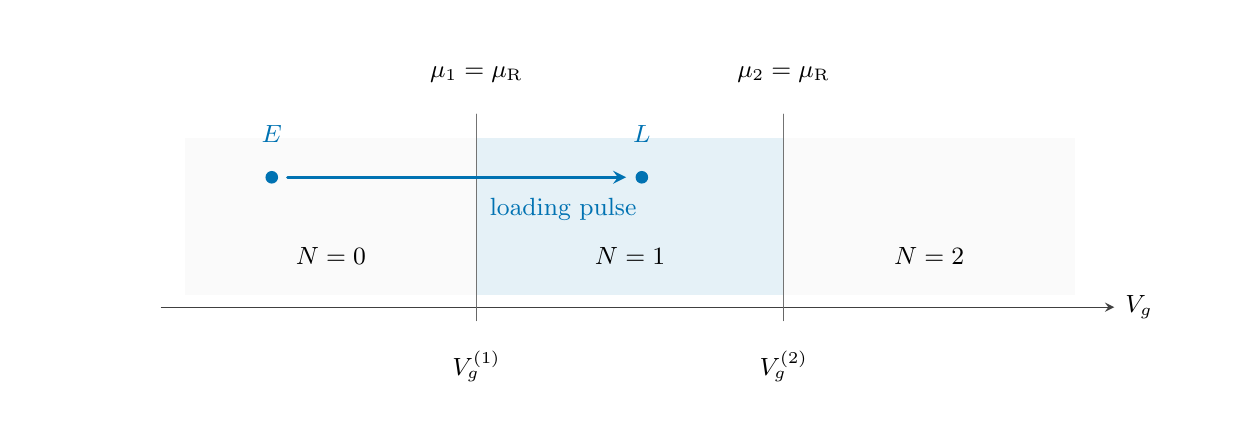
\begin{tikzpicture}[
 x=1mm,y=1mm,>=stealth,line cap=round,line join=round,
 every node/.style={font=\small,inner sep=1pt}
]
 \path[use as bounding box] (0,3) rectangle (150,52);

 % Charge sectors at a fixed reservoir chemical potential.
 \fill[black!2] (20,18) rectangle (133,38);
 \fill[loadingGate!10] (57,18) rectangle (96,38);
 \draw[black!55,line width=0.5pt] (57,16.5)--(57,41);
 \draw[black!55,line width=0.5pt] (96,16.5)--(96,41);
 \node at (38.5,23) {$N=0$};
 \node at (76.5,23) {$N=1$};
 \node at (114.5,23) {$N=2$};
 \node at (57,46) {$\mu_1=\mu_{\mathrm R}$};
 \node at (96,46) {$\mu_2=\mu_{\mathrm R}$};

 % A pulse crosses the first threshold and stops inside the N=1 interval.
 \fill[loadingGate] (31,33) circle (0.8);
 \fill[loadingGate] (78,33) circle (0.8);
 \draw[->,loadingGate,line width=1.05pt] (33,33)--(76,33);
 \node[text=loadingGate] at (31,38.5) {$E$};
 \node[text=loadingGate] at (78,38.5) {$L$};
 \node[text=loadingGate,fill=loadingGate!10,inner sep=0.5pt]
      at (68,29) {loading pulse};

 % Gate axis and charge-degeneracy voltages.
 \draw[->,black!75,line width=0.5pt] (17,16.5)--(138,16.5);
 \node[anchor=west] at (139,16.5) {$V_g$};
 \foreach \tickX in {57,96}{
  \draw[black!60,line width=0.4pt]
       (\tickX,16.5)--(\tickX,14.8);
 }
 \node at (57,9) {$V_g^{(1)}$};
 \node at (96,9) {$V_g^{(2)}$};
\end{tikzpicture}
\endgroup
